\documentclass[a4paper,12pt]{scrartcl}
\usepackage[utf8]{inputenc}
\usepackage[ngerman]{babel}
\usepackage{graphicx}
\usepackage{url}

% Title Page
\title{Zwischenbericht Master-Projekt Bildverarbeitung}
\subtitle{SoSe 2015}
\author{Dorothee Geiser, Niels Porsiel}
\date{\today}


\begin{document}

\maketitle
\thispagestyle{empty}
\vspace{0.3\textheight}

\begin{abstract}
Im laufe des Semesters haben wir uns mit Scale-Invariant Feature Transform (kurz SIFT)
beschäftigt. Dabei haben wir uns am Paper \textit{Distinctive Image Features from Scale-
Invariant Keypoints} von David G. Lowe \cite{Lowe} orientiert. Unsere Aufgabe war es zu 
versuchen, SIFT nachzubauen. Dieser Zwischenbericht soll nun einen Überblick darüber 
geben, was wir geschafft haben.
\end{abstract}

\newpage
\tableofcontents
\newpage

\section{Unser Code}
\subsection{Keypoint-Erkennung}
Die erste Aufgabe war das Erkennen von Keypoints in einem Grauwertbild. Gesucht sind 
prominente Hell-/Dunkel-Kontraste, die (skaleninvariant) wiederzufinden sein sollen. Um 
dies zu bewerkstelligen, bauen wir, nach Vorgabe von Kapitel 3 von Lowe \cite{Lowe}, ein 
Set aus Oktaven mit je fünf Skalen auf. Die Anzahl Oktaven ergibt sich dabei aus dem 
binären Logarithmus des Minimums von Höhe und Breite des Ausgangsbildes minus drei (= die 
maximale Anzahl mit der das Bild um den Faktor vier verkleinert werden kann). Bevor die 
Oktaven erzeugt werden, muss festgelegt werden, ob das Ausgangsbild auf die doppelte 
Größe skaliert wird um eine extra Oktave zu erzeugen. Dies geschieht bei uns mittels des 
boolschen Parameters \url{double_image_size}, der dem Programm bei Aufruf übergeben 
werden kann (default ist true). \\ \ \\
Zum Aufbau der Oktaven wird das (eventuell skalierte) Ausgangsbild mithile von einem 
Gaußfilter gefaltet und diese Operation so oft wiederholt, bis die festgelegte Anzahl 
Bilder pro Oktave (bei uns fünf) erreicht ist. Das letzte und unschärfste Bild einer 
Oktave wird skaliert, so dass es nur noch die Hälfte in Höhe und Breite misst, also um 
den Faktor 4 verkleinert und als Ausgangsbild für die nächste Oktave verwendet. \\
Die Berechnung der Standardabweichung des Gaußfilters kann dabei iterativ oder absolut 
durchgeführt werden. Bei der iterativen Berechnung wird die Standardabweichung abhängig 
von der Standardabweichung des Bildes aus der letzten Iteration mittels der Formel 
$\sqrt{\sigma_{total}^2 - \sigma_{last}^2}$ berechnet, wobei $\sigma_{last} = 
k^{(i-1)}*\sigma$ und $\sigma_{total} = \sigma_{last}*k$. $k$ wird im Paper von Lowe als
$k=2^{(1/s)}$ definiert, für $s$ haben wir 2 als Wert gewählt, $i$ ist die Iteration in 
der aktuellen Oktave und $\sigma$ kann auch als Aufrufparameter an das Programm übergeben 
werden (default ist 1.0). Die absolute Methode verwendet zur Berechnung immer das 
Ausgangsbild der aktuellen Oktave. %um das nächste Bild zu erzeugen. 
Die Standardabweichung berechnet sich hierbei durch die Formel $k^i*\sigma$. Die Wahl der 
Methode wird über die boolsche Variable \url{iterative_interval_creation} gesteuert und 
kann dem Programm auch beim Aufruf übergeben werden (default ist true). \\ \ \\
Aus zwei benachbarten Bildern jeder Oktave wird jeweils ein sogenannter 
Difference-of-Gaussian (DOG) gebildet. Dafür wird die Differenz der Grauwerte in jedem 
Pixel errechnet und aus den resultierenden Werten ein neues Bild erzeugt. Sobald 
mindestens drei DOGs vorhanden sind, wird in diesen nach Extrempunkten gesucht. Dies 
geschieht, indem der Grauwert jedes Pixels mit dem seiner umliegenden Nachbarn verglichen 
wird; 8 direkte Nachbarn im eigenen DOG und jeweils 9 im darüber und darunter liegenden 
(siehe Abbildung 2 im Paper  von Lowe). Pixel, die am Rand des aktuellen DOGs oder im 
ersten / letzten DOG liegen, werden dabei ignoriert. \\
Ist der Wert des Pixels höher oder niedriger als der aller seiner Nachbarn und größer als 
ein festgelegter Grenzwert \url{dog_threshold} (Aufrufparameter, default ist 5.0), wird 
er als Keypoint erkannt.  Der Vergleich wird in der Inline Funktion \url{localExtremum} 
durchgeführt, die als Parameter einen Pointer auf einen Standardvektor \url{dog} aus 
vigra-Multiarrays und drei Integer $i$, $x$ und $y$ für den aktuellen Pixel annimmt. 
Dabei sind $x$ und $y$ die Koordinaten des Pixels im DOG und $i$ der Index für den 
DOG-Vektor, in welchem sich der Pixel befindet.  Die Funktion liefert den boolschen Wert
true zurück, wenn der Pixel ein Extrempunkt ist (sonst false).
\\ \ \\
Die so erkannten Keypoints sieht man in Abbildung \ref{Bild1}.

% Umschreibung unseres Codes
% 
%     bool double_image_size: legt fest, ob das Inputbild vorher auf doppelte Größe skaliert werden soll (extra Oktave)
% 
%     also vorher erwähnen, dass wir Oktaven brauchen und warum
% 
%     Anzahl Oktaven: Binärer Logarithmus des Minimums aus Höhe und Breite des Bildes - 3
% 
%     Begründung für bestimmte Anzahl Oktaven, Vor-/Nachteile von mehr / weniger
% 
%     s=2, k=2^(1/s) (wird irgendwie für die sigma Berechnung gebraucht -> im Paper nachgucken)
% 
%     Wozu wird das Sigma gebraucht?
% 
%     intervals = s+3 (Anzahl Bilder pro Oktave)
% 
%     das gleiche wie für die Anzahl Oktaven
% 
%     bool iterative_interval_creation: Iterative Berechnung des Sigma-Wertes für die DOGs oder absolute Berechnung
% 
%     wo liegt der Unterschied?
% 
%     iterative Berechnung: Ausgangsbild wird mit Sigma geglättet, geglättetes Bild wird als Ausgangsbild für nächste Stufe genommen usw...
% 
%     absolute Berechnung: Ausgangsbild wird immer als Ausgangsbild genommen und mit verschiedenen Sigmas die Skalen erzeugt
% 
%     gaussianSmoothing: vigra-Funktion, die ein Bild und einen Sigma-Wert annimmt, dieses mit Gauss und gewählter Standardabweichung glättet und das Ergebnisbild ausgibt
% 
%     wozu glätten?
% 
%     resize: nach jeder Oktave wird das Bild um ein Viertel verkleinert: Halbe Höhe, halbe Breite
% 
%     warum?
% 
%     wenn mindestens 3 DOGs vorhanden sind: Suche nach Extrema
% 
%     warum 3?
% 
%     keine Randpixel: for-Schleifen von x=1,y=1 bis x=width-1, y=height-1
% 
%     Pixel werden mit insgesamt 26 Nachbarn verglichen:
% 
%     8 Nachbarn auf demselben DOG
% 
%     9 Nachbarn auf jeweils dem DOG dadrüber und dadrunter
% 
%     -> Aufruf der Inline Funktion localExtremum mit dem DOG Array dieser Oktave, der momentanen Skala (i), x und y
% 
%     Wert des zu prüfenden Pixel muss entweder höher oder niedriger als der aller seiner Nachbarn sein -> Berechnung geht weiter, sonst Abbruch

\begin{figure}[htbp]
  \centering
  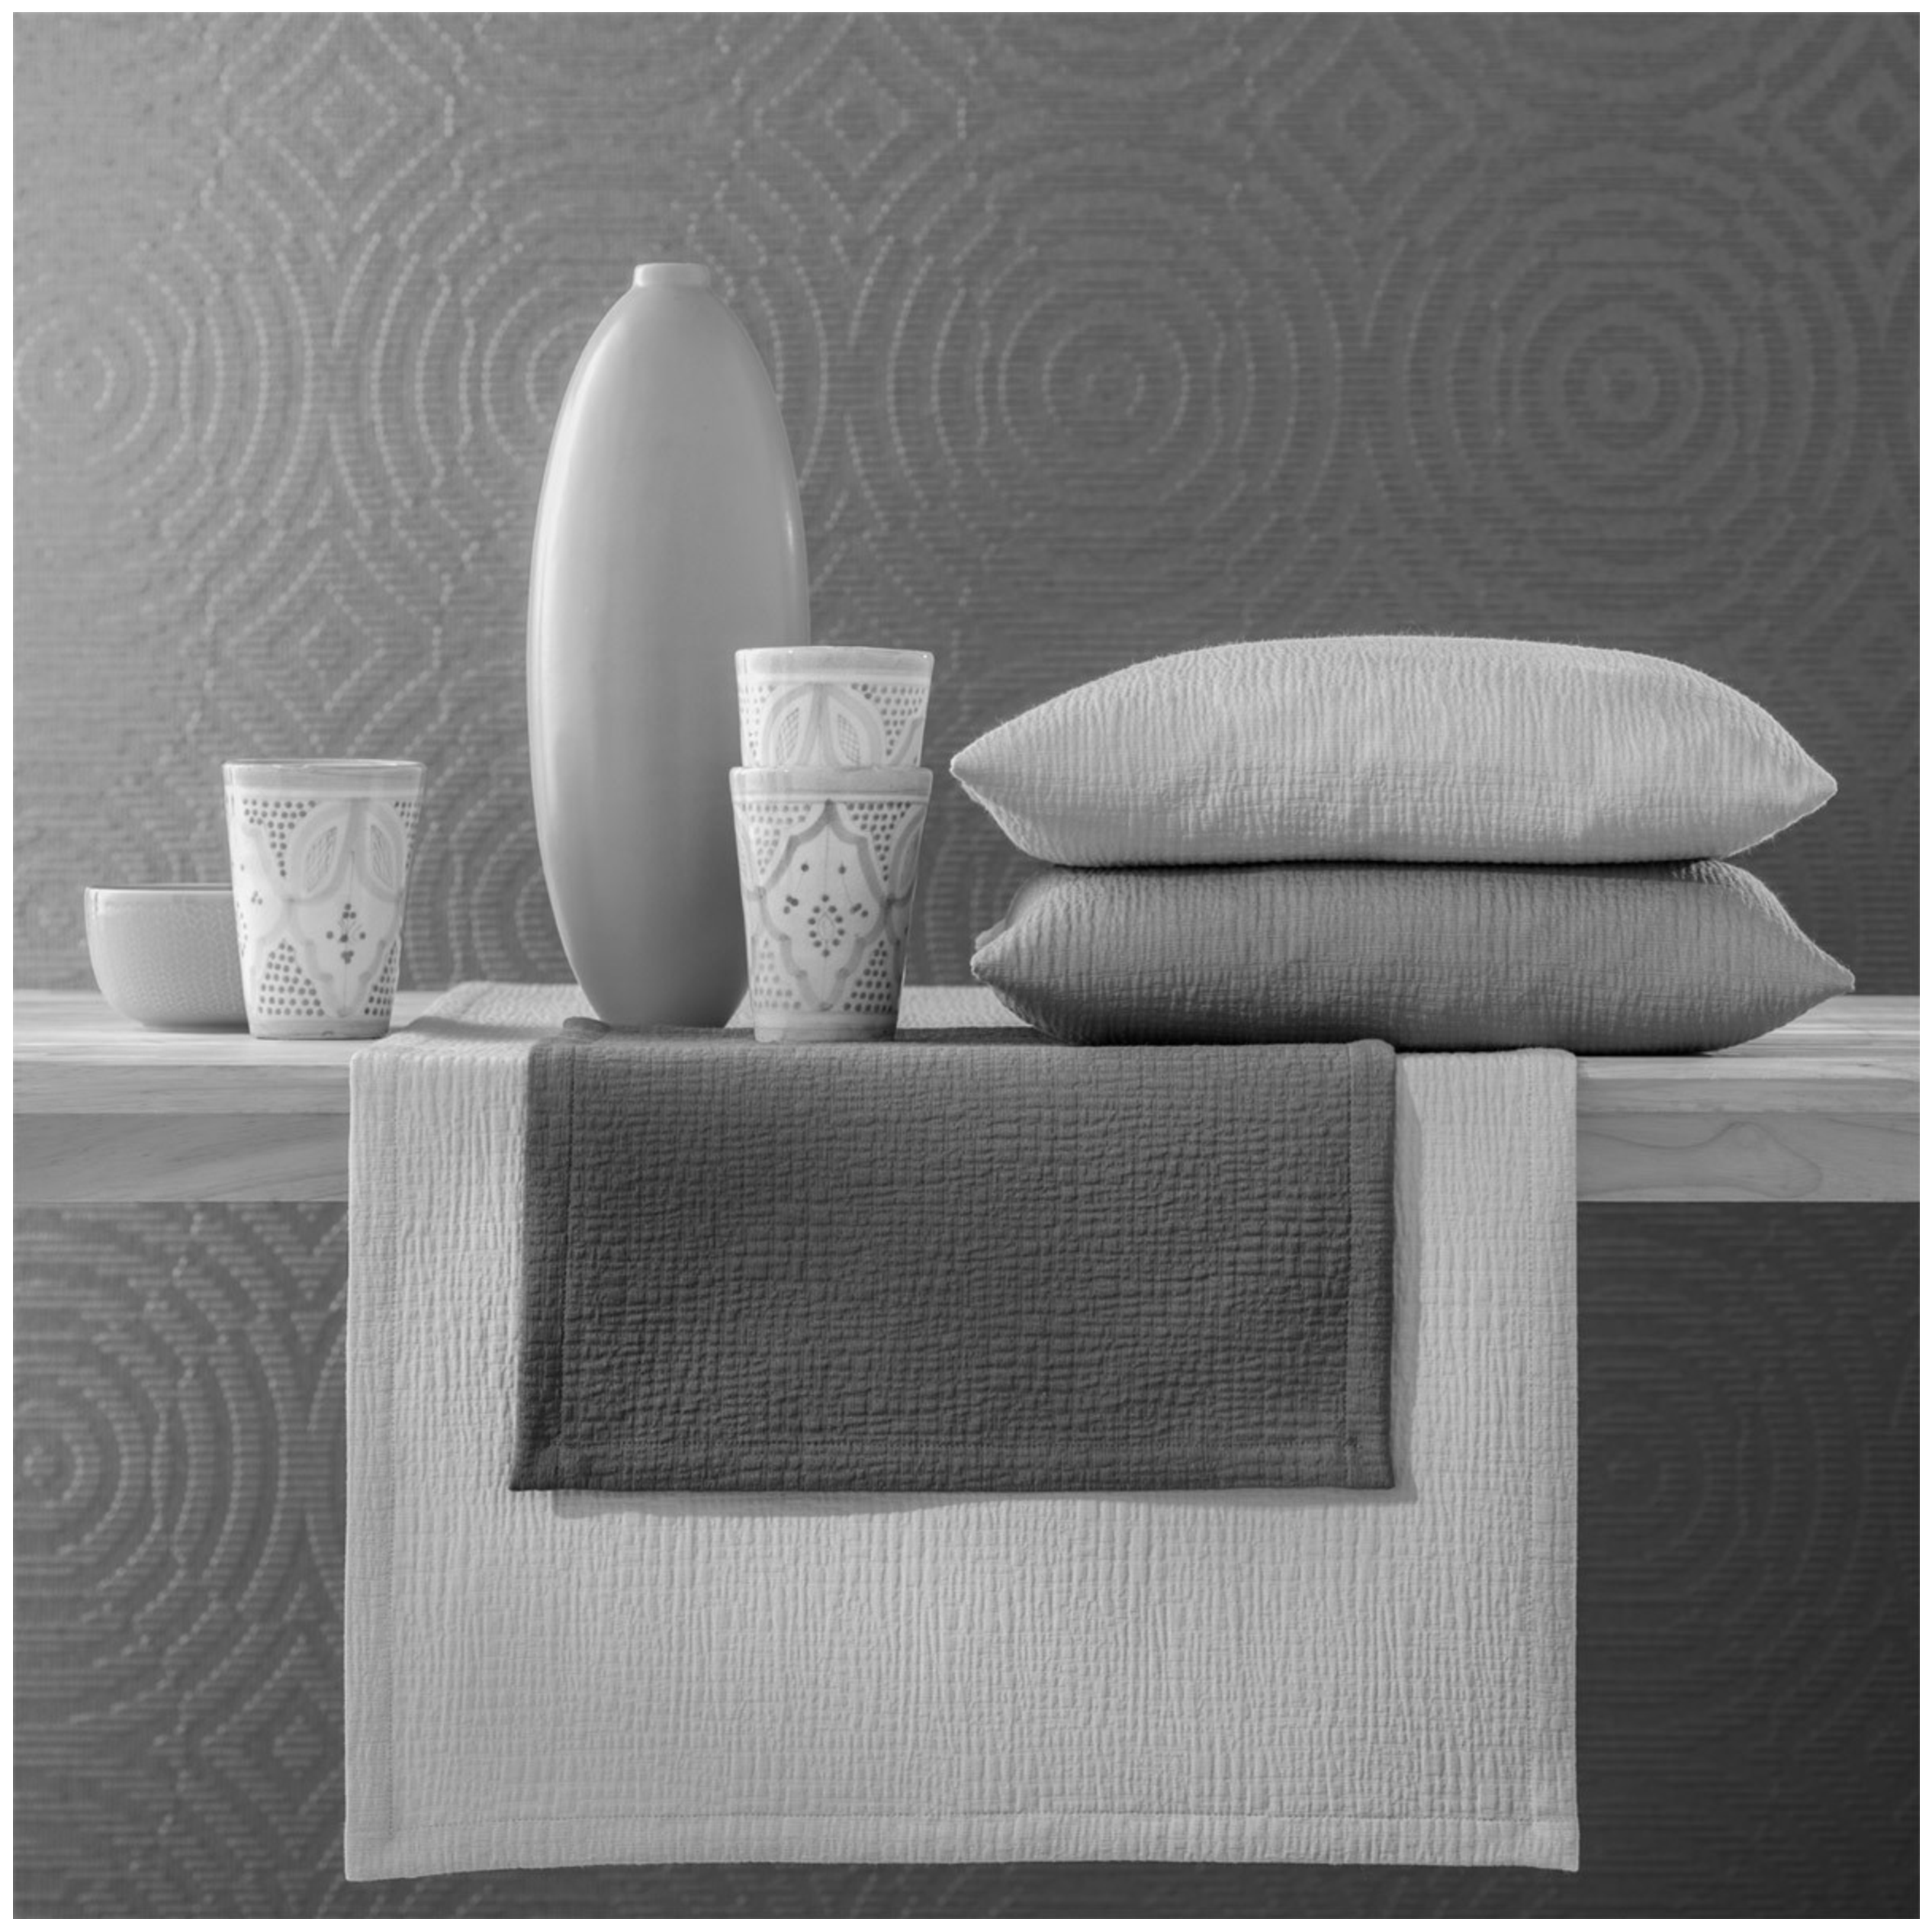
\includegraphics[width=0.45\textwidth]{bild}
  \fbox{ 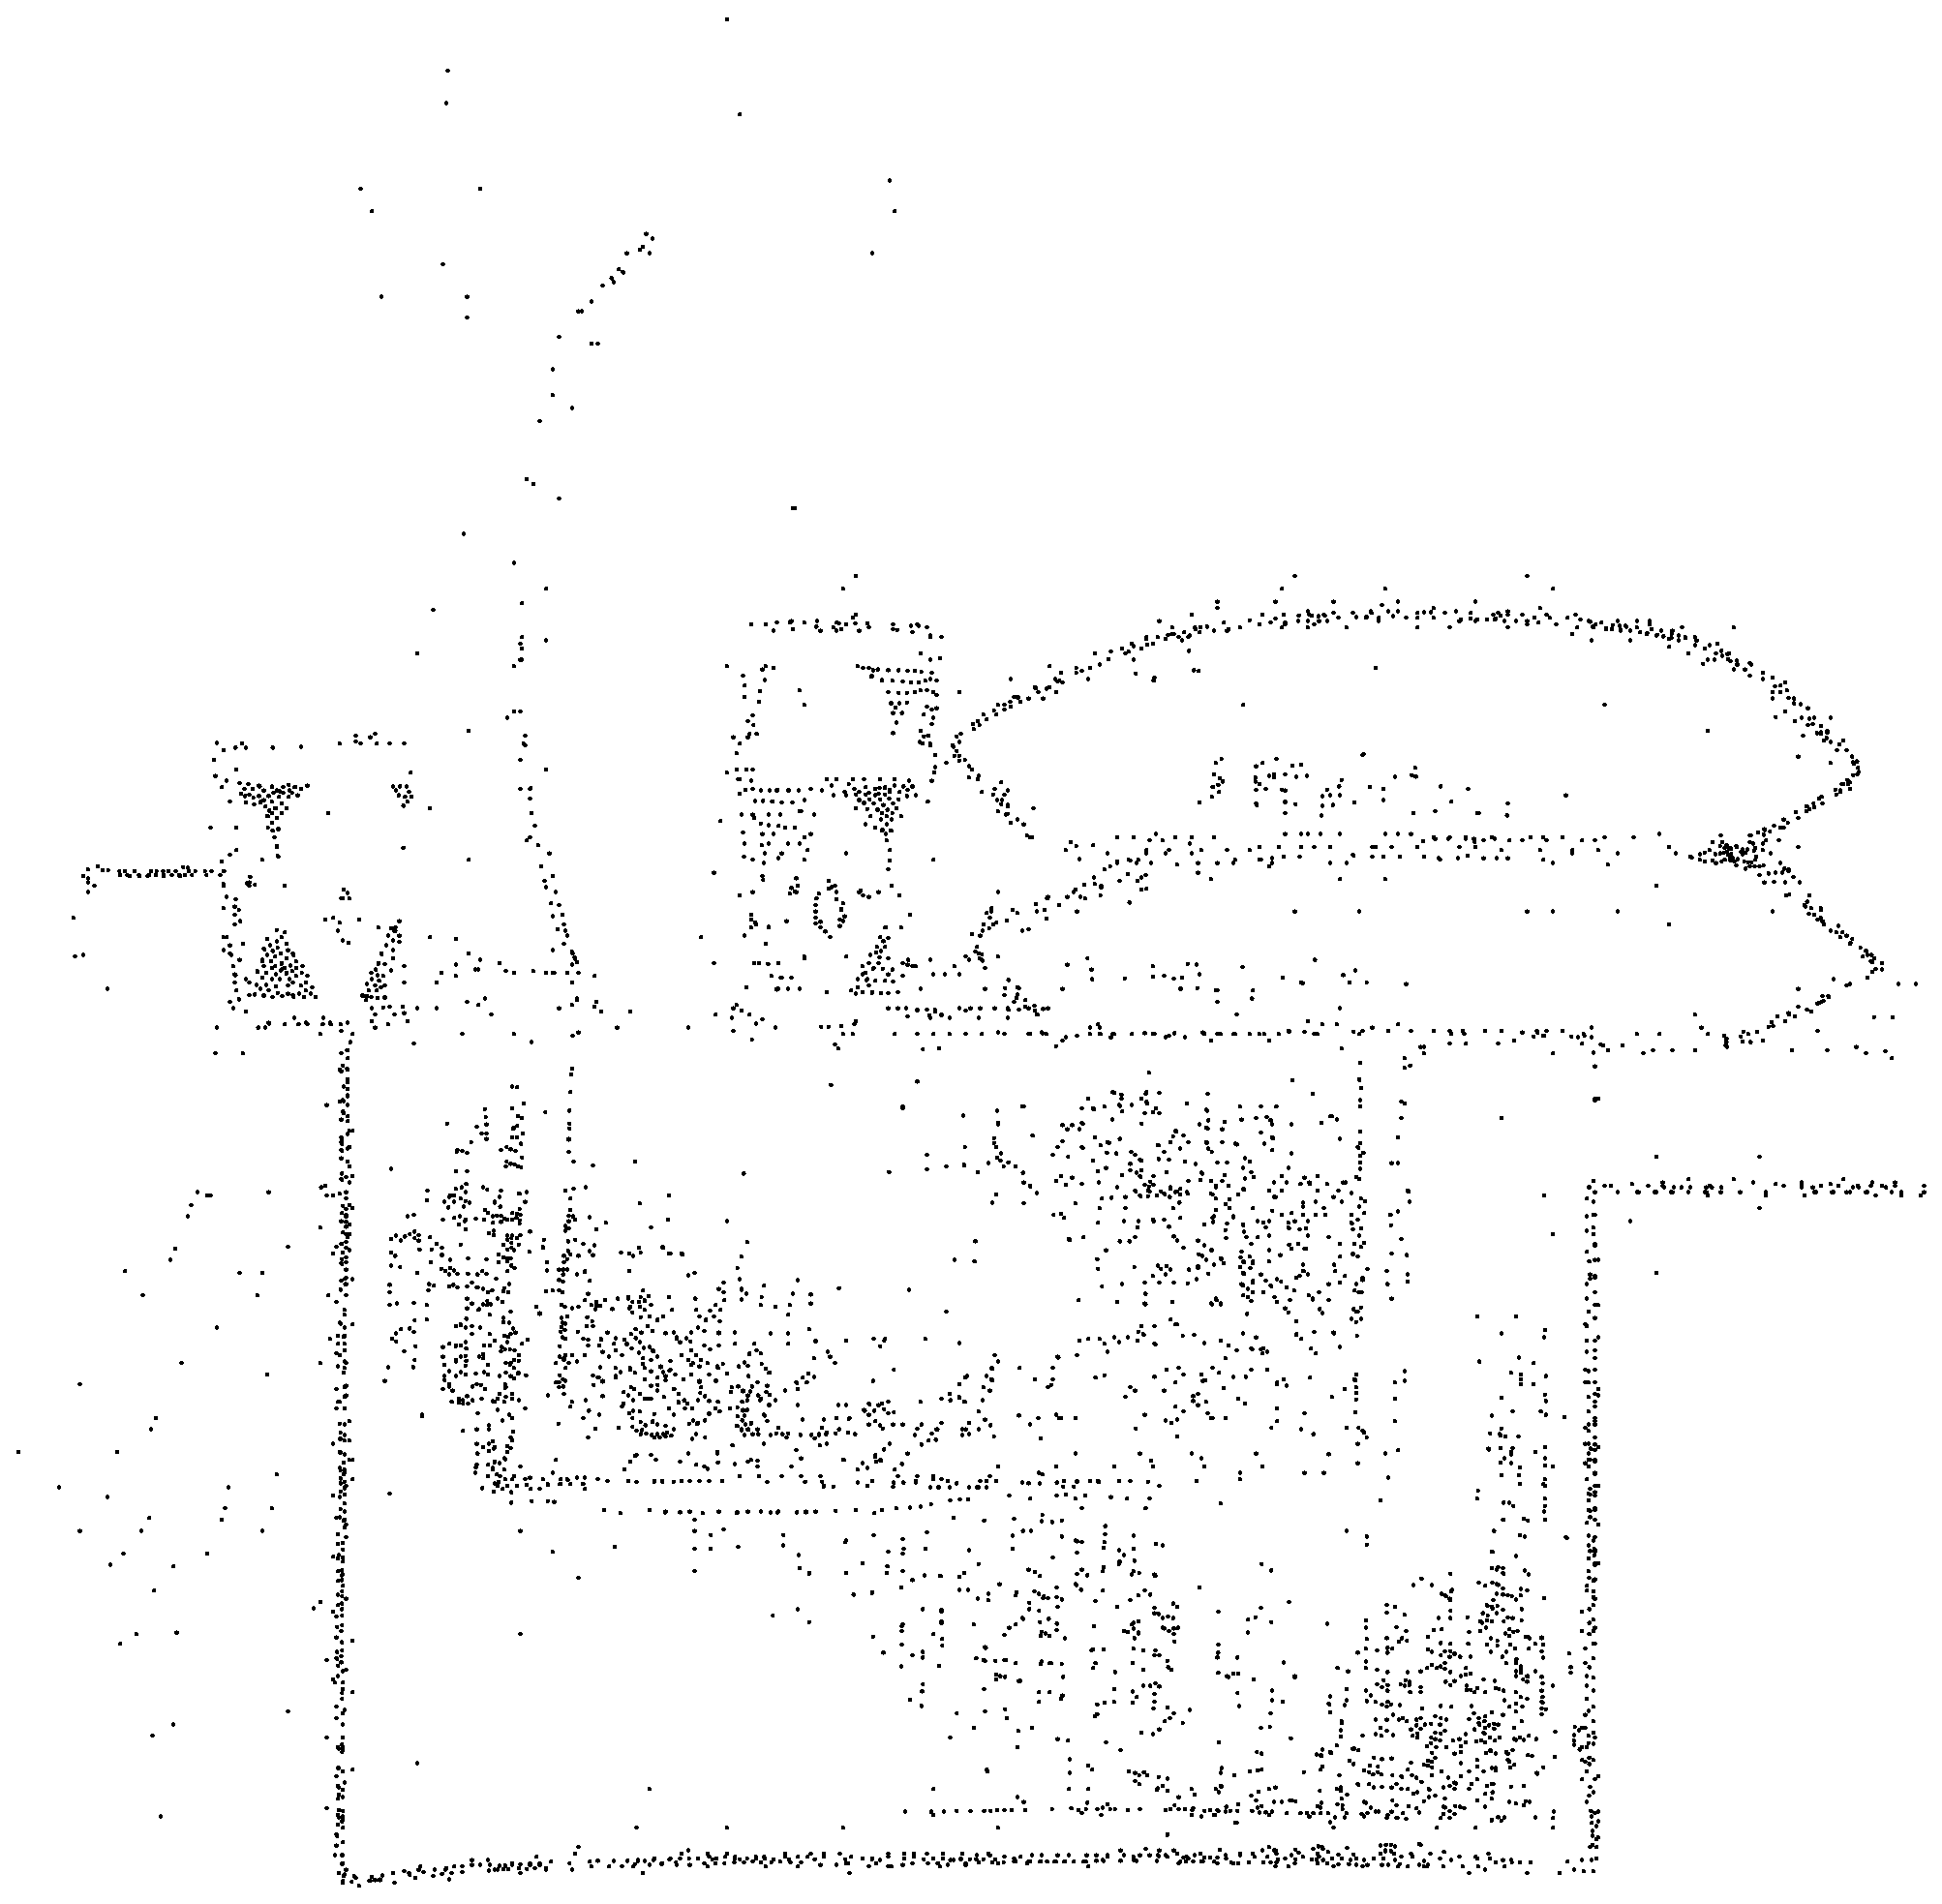
\includegraphics[width=0.45\textwidth]{1Extrema} }
  \caption{Keypoint-Erkennung. Links das Original, rechts die erkannten Keypoints.}
  \label{Bild1}
\end{figure}

\subsection{Keypoint-Reduktion und Verschiebung auf Subpixel-Ebene}
Im nächsten Schritt sollte die Anzahl der erkannten Keypoints reduziert werden und [...].
Das Ergebnis sieht man in Abbildung \ref{Bild2}.

%     Grauwert des Pixels muss größer als dog_threshold (5) sein (Parameter)
% 
%     warum?
% 
%     Verschiebung der gefunden Extrema auf Subpixel-Ebene:
% 
%     warum?
% 
%     -> Aufruf der Funktion subpixel mit dem DOG Array dieser Oktave, der momentanen Skala (i), x, y, threshold, ratio, Höhe-1 und Breite-1 des DOGs, Offset in x,y,z-Richtung die als Ausgabe-Parameter dienen
% 
%     Berechnung der partiellen ersten Ableitung in die 3 Dimensionen x,y,sigma
% 
%     Berechnung der partiellen zweiten Ableitung in alle 3 Dimensionen
% 
%     Hesse-Matrix aus den zweiten Ableitungen bilden
% 
%     Spur der Hesse-Matrix zum Quadrat geteilt durch die Determinante der Hesse-Matrix
% 
%     Eliminierung von Extrema, wenn Verhältnis (ratio(10)) der Hauptkrümmung unter gegebenem Wert liegt: ((ratio-1)^2)/ratio
% 
%     lineare Berechnung von Vektor der ersten Ableitungen mit der Hesse-Matrix ergibt Offset
% 
%     Eliminierung von Extrema mit schwachem Kontrast unter gegebenem Threshold (0.03*256)
% 
%     Offset in X und/oder Y Richtung wird ignoriert, wenn Offset > 0.5

\begin{figure}[htbp]
  \centering
  \fbox{ 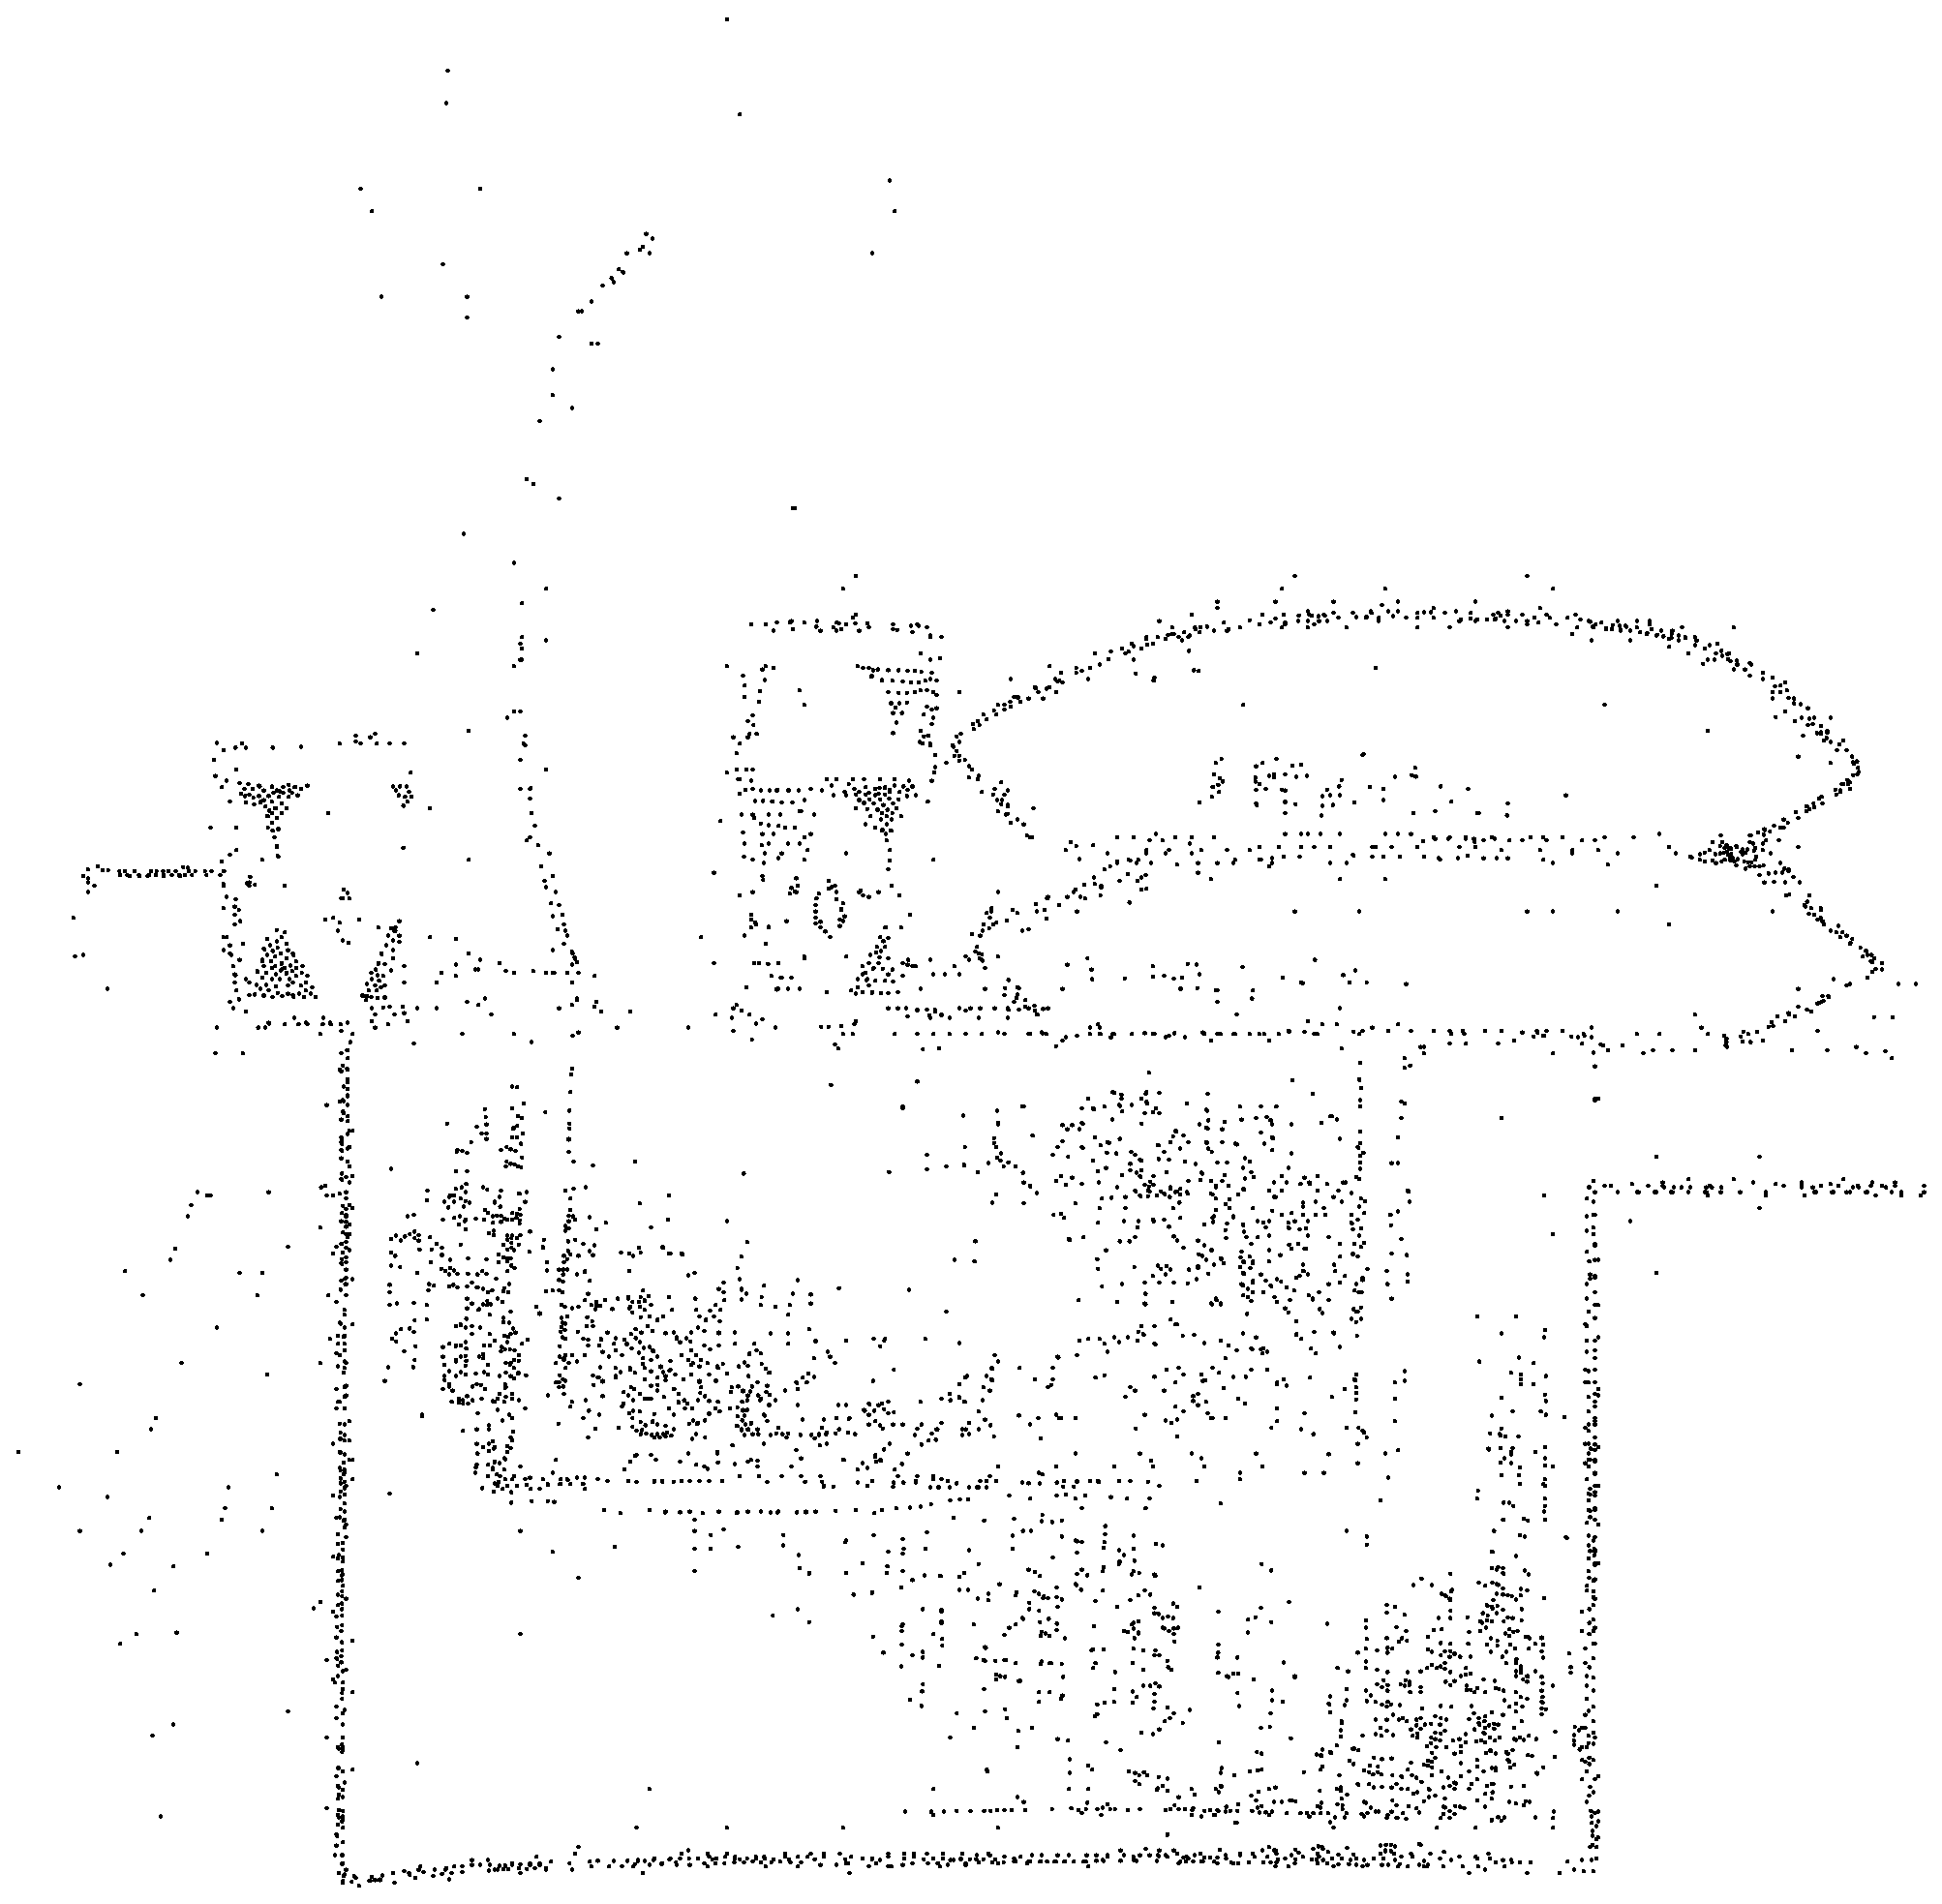
\includegraphics[width=0.45\textwidth]{1Extrema} }
  \includegraphics[width=0.45\textwidth]{4RechteckemHkorrigiert} 
  \caption{Keypoint-Reduktion und Verschiebung auf Subpixel-Ebene. Links die vorher erkannten
  Keypoints, rechts die jetzt erkannte, [...] geringere Menge.}
  \label{Bild2}
\end{figure}

\subsection{Keypoint-Orientierung}
Dann folgte die Keypoint-Orientierung. Das Ergebnis sieht man in Abbildung \ref{Bild3}.

%     Sigma des DOGs rausfinden, aus der der aktuelle Keypoint stammt
% 
%     wozu braucht man das sigma? [steht oben]
% 
%     Orientation des Keypoints berechnen:
% 
%     wozu ist das wissen über die orientierung gut?
% 
%     -> Aufruf der Funktion orientation mit dem Octave Array dieser Oktave, der Skala (Sigma), x und y, angle und angle2 sind die Rückgabeparameter der Funktion
% 
%     Prüfung, ob 8 Pixel Abstand zum Rand des Bildes in x und y-Richtung vorhanden sind, sonst Eliminierung
% 
%     Für die benachbarten 8x8 Pixel des Keypoints wird die Magnitude und der Winkel berechnet
% 
%     Der Abstand, der benachbarten Pixel zum Keypoint wird mit einem Gauss gewichtet (8/3, wegen 8 Pixel Radius) und mit der Magnitude multipliziert. Dieser Wert wird je nach berechnetem Winkel in ein Histogramm mit 36 Fächern eingetragen, wobei jedes Fach für 10° steht
% 
%     Nach Befüllung des Histogramms wird das Element mit dem größten Wert gesucht
% 
%     Falls es ein zweites Element gibt, welches mindestens 80% des Wertes des größten Elements erreicht, wird dieses ebenfalls verwendet und ein zweiter Keypoint mit denselben Koordinaten aber mit dem anderen Winkel erzeugt
% 
%     Durch eine Parabelfunktion wird mit dem größten Element und seinen beiden Nachbarn mit den Winkeln jeweils um 5° (quasi in die Mitte des 10° Feldes) verschoben der genaue Winkel berechnet und zurück gegeben
% 
%     Falls ein zweites Element gefunden wurde, wird die Operation erneut mit diesem Element ausgeführt

\begin{figure}[htbp]
  \centering
  \includegraphics[width=0.45\textwidth]{4RechteckemHkorrigiert} 
  \includegraphics[width=0.45\textwidth]{5RechteckOrientierung}  
  \caption{Keypoint-Orientierung. Links ohne, rechts mit Orientierung.}
  \label{Bild3}
\end{figure}

\subsection{Keypoint Deskriptoren}
Schlussendlich kamen noch die Keypoint Deskriptoren.

%     Deskriptor des Keypoints erstellen:
% 
%     wozu sind die gut?
% 
%     -> Aufruf der Funktion keypoint mit dem Octave Array dieser Oktave, der Skala(Sigma), x, y und Winkel, feature ist der Deskriptor als Array und der Rückgabewert der Funktion
% 
%     Prüfung, ob 16 Pixel Abstand zum Rand des Bildes in x und y-Richtung vorhanden sind, sonst Eliminierung
% 
%     Ein SplineImageView wird für das verwendete Bild erzeugt
% 
%     Der Keypoint wird um seine Orientierung gedreht und für die benachbarten 16x16 Pixel werden wieder Magnitude und Winkel berechnet
% 
%     Der Abstand, der benachbarten Pixel zum Keypoint wird mit einem Gauss gewichtet (8) und mit der Magnitude multipliziert. Dieser Wert wird je nach berechnetem Winkel in ein Histogramm mit 8 Fächern eingetragen, wobei jedes Fach für 45° steht
% 
%     Die Pixel werden je nach Lage in Regionen eingeteilt, für die es jeweils ein Histogramm gibt. Eine Region besteht aus 4x4 Pixeln, also gibt es 16 Regionen. Jede Region hat ein Histogramm mit 8 Fächern.
% 
% 
%     ToDo: Die Werte von Pixeln müssen auch in Histogramme benachbarter Regionen eingetragen werden und mit der Distanz dazu gewichtet werden [evtl einen Abschnitt tiefer]
% 
% 
%     Die Histogramme sind die Deskriptoren der Keypoints.

\section{Vergleich des Erreichten mit der Vorgabe}
Im Vergleich mit dem, was Lowe \cite{Lowe} getan hat ...

%%%% Literatur
\newpage
\begin{thebibliography}{------}
\bibitem[Lowe04]{Lowe}
  David G. Lowe: {\em Distinctive Image Features from Scale-Invariant Keypoints}. 
  International Journal of Computer Vision 60(2): pp 91-110 (2004)
\end{thebibliography}

\end{document}          
